\chapter{Screenshots of the Web Portal}

\begin{enumerate}
\item Home Page of the Web Portal for NGO's Registration and other functionalities
\begin{figure}[here]
\begin{center}   
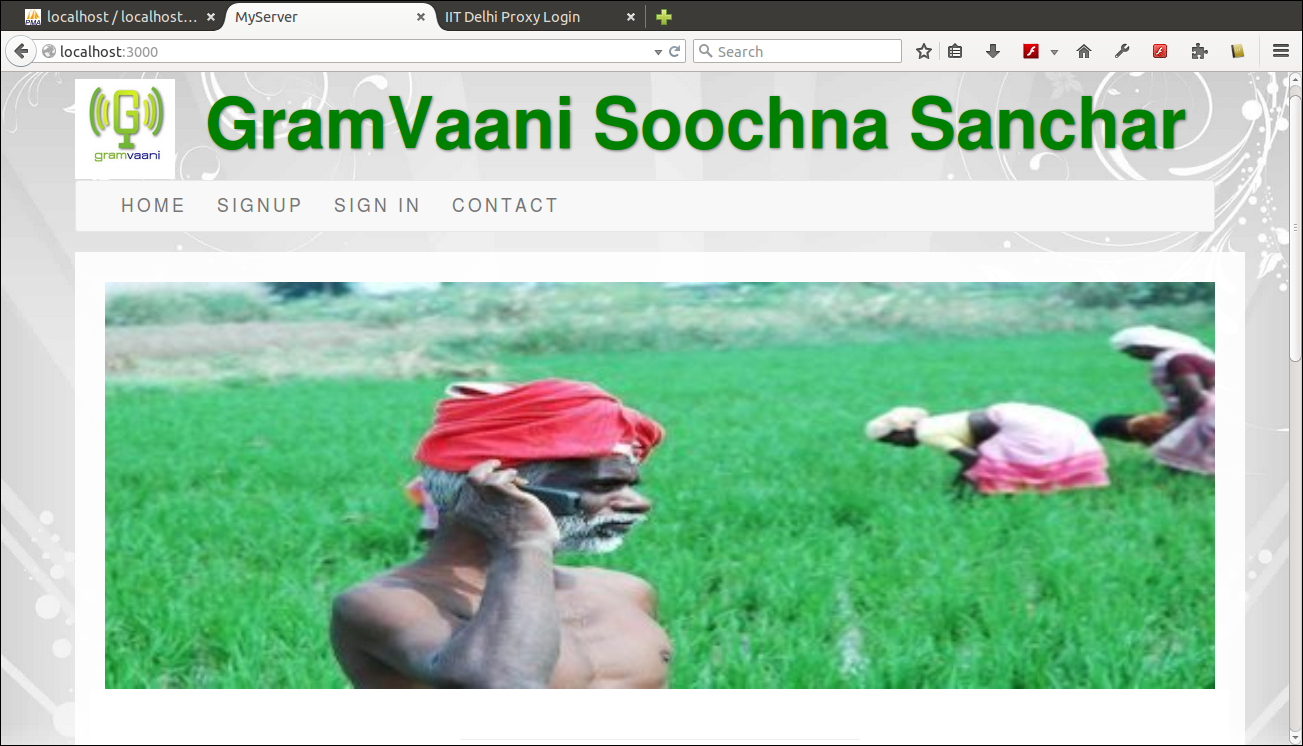
\includegraphics[scale=0.3]{w1}
\caption{GramVaani Soochna Sanchar Home Page}
\label{fig:w1}
\end{center}
\end{figure}


\item NGO's Login Page
\begin{figure}[here]
\begin{center}   
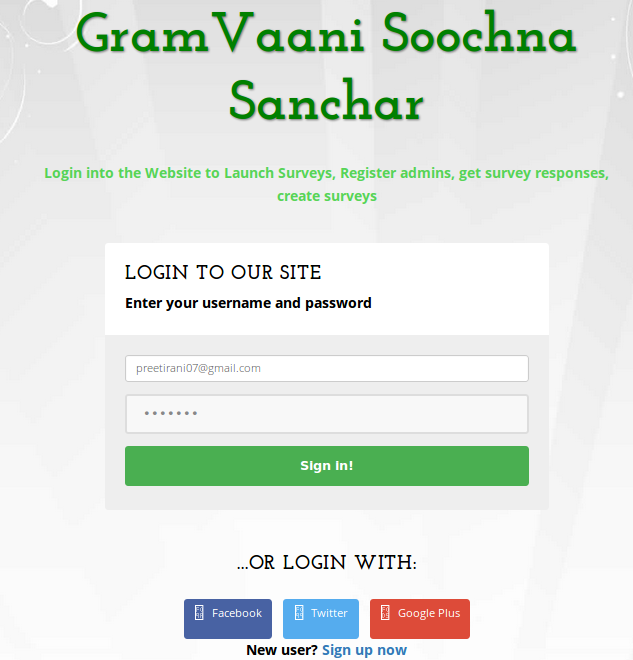
\includegraphics[scale=0.3]{w10}
\caption{NGO's Login Page}
\label{fig:w10}
\end{center}
\end{figure}



\item Use cases provided to the NGO users
\begin{figure}[here]
\begin{center}   
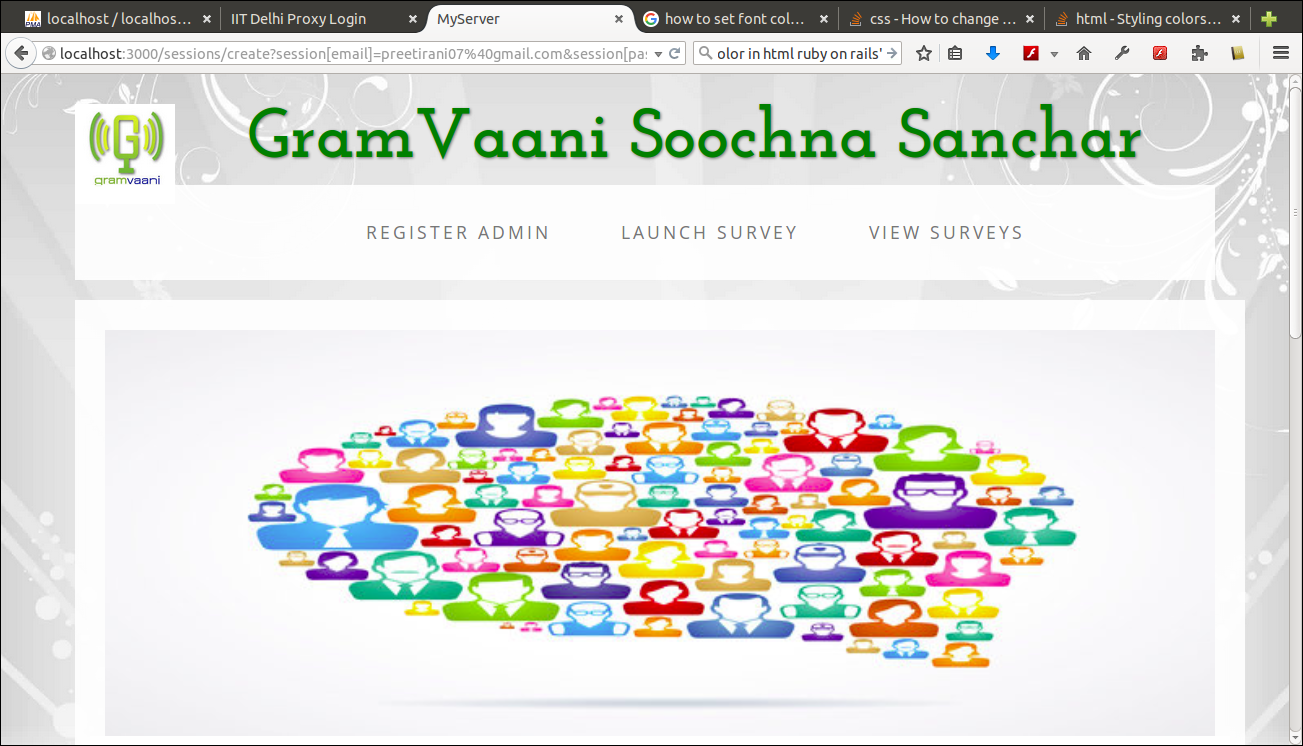
\includegraphics[scale=0.3]{w14}
\caption{Use Cases of NGO Personnel}
\label{fig:w14}
\end{center}
\end{figure}



\item Web Online form for Admins Registration and Authentication
\begin{figure}[here]
\begin{center}   
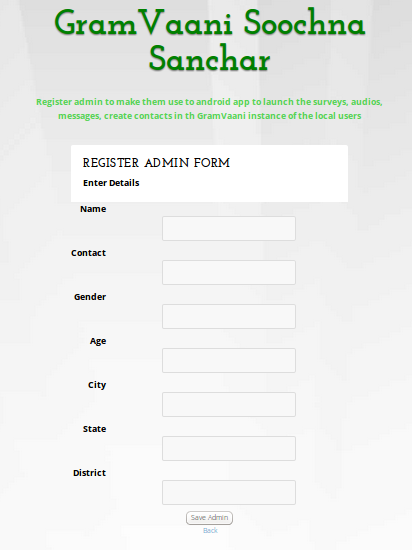
\includegraphics[scale=0.3]{w15}
\caption{Admin's Registration Form}
\label{fig:w15}
\end{center}
\end{figure}




\item NGO Personnel can launch a particular survey for a particular district.
\begin{figure}[here]
\begin{center}   
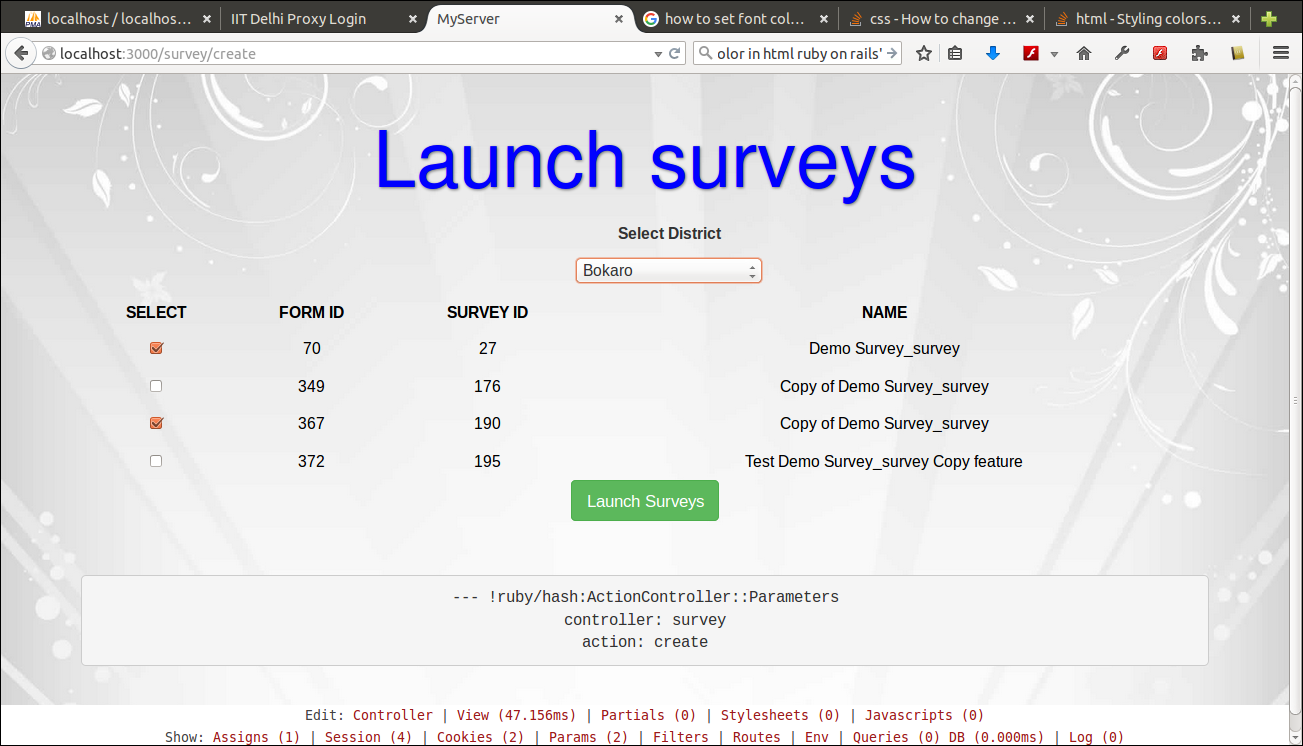
\includegraphics[scale=0.3]{w16}
\caption{Launch Survey in a District}
\label{fig:w16}
\end{center}
\end{figure}


\item NGO Personnel can view all the active surveys along with viewing current responses and survey questions.
\begin{figure}[here]
\begin{center}   
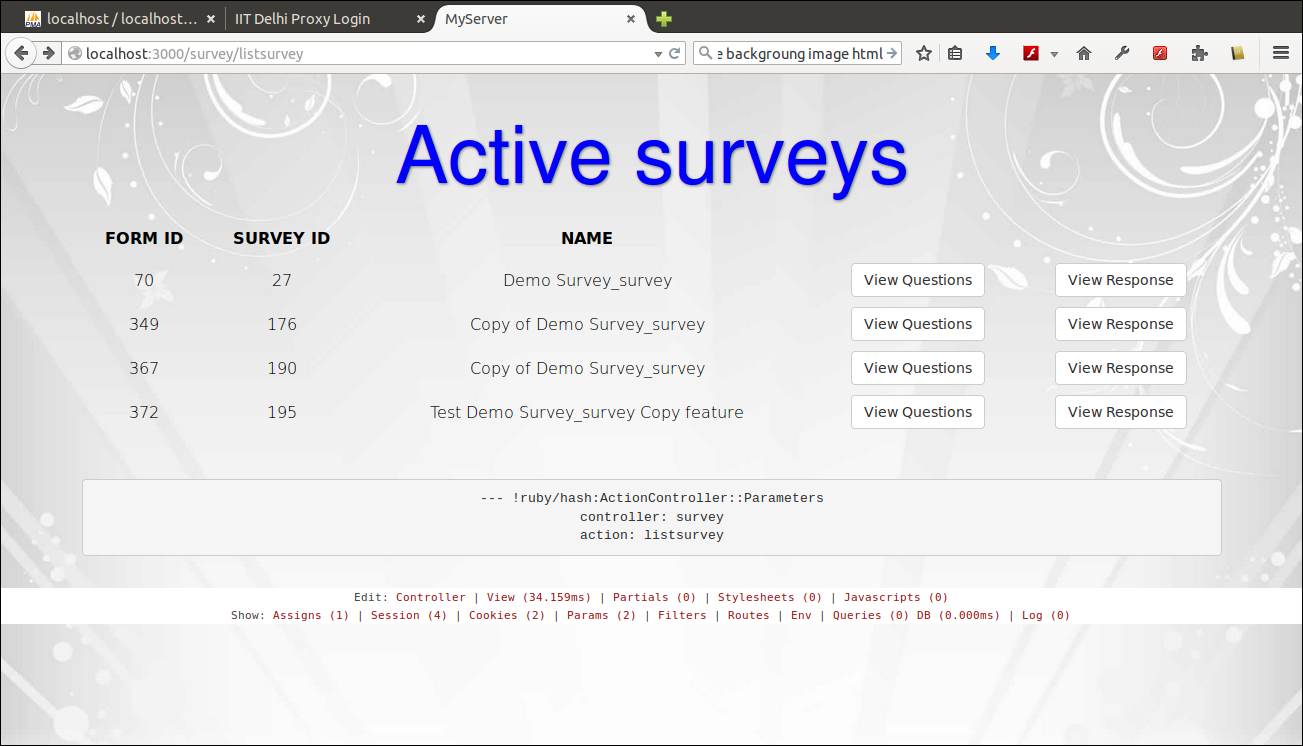
\includegraphics[scale=0.3]{w13}
\caption{View Active Surveys}
\label{fig:w13}
\end{center}
\end{figure}


\item NGO Personnel can view the responses of the active survey.
\begin{figure}[here]
\begin{center}   
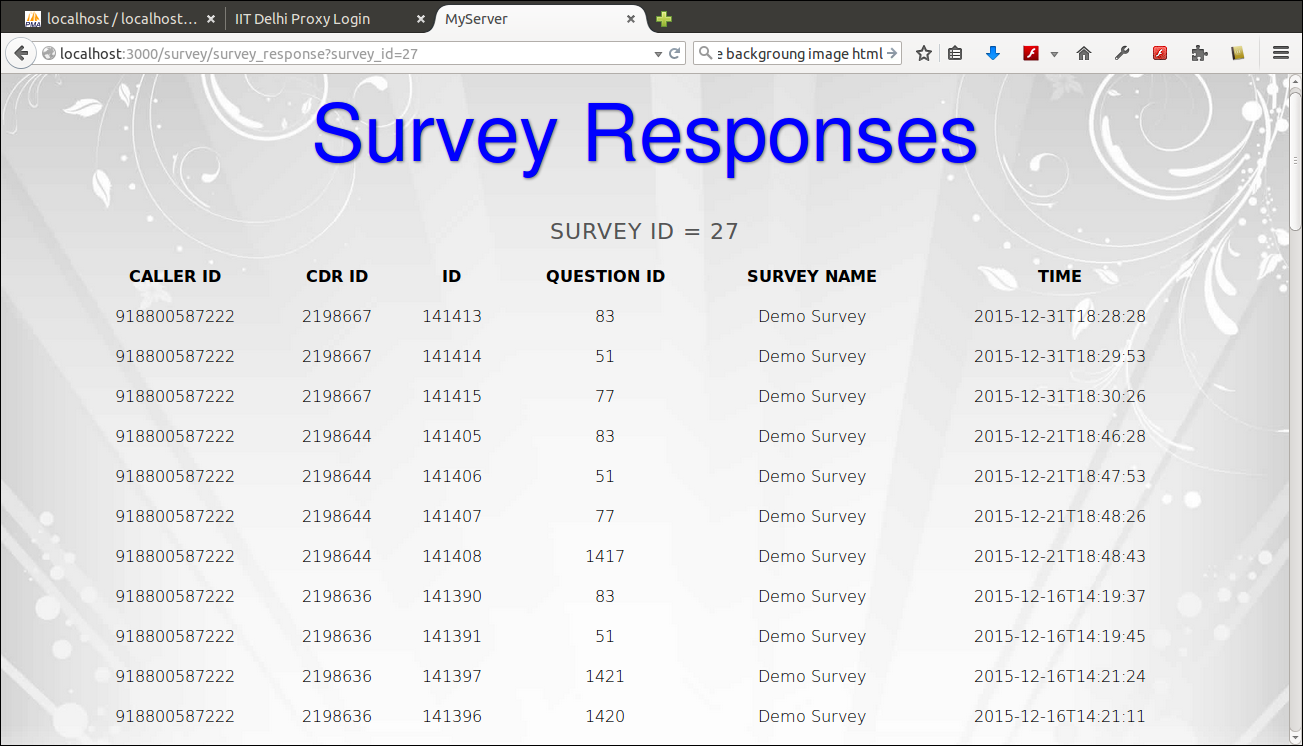
\includegraphics[scale=0.3]{w11}
\caption{View Active Survey Responses}
\label{fig:w11}
\end{center}
\end{figure}


\item NGO Personnel can view the text questions of the active survey.
\begin{figure}[here]
\begin{center}   
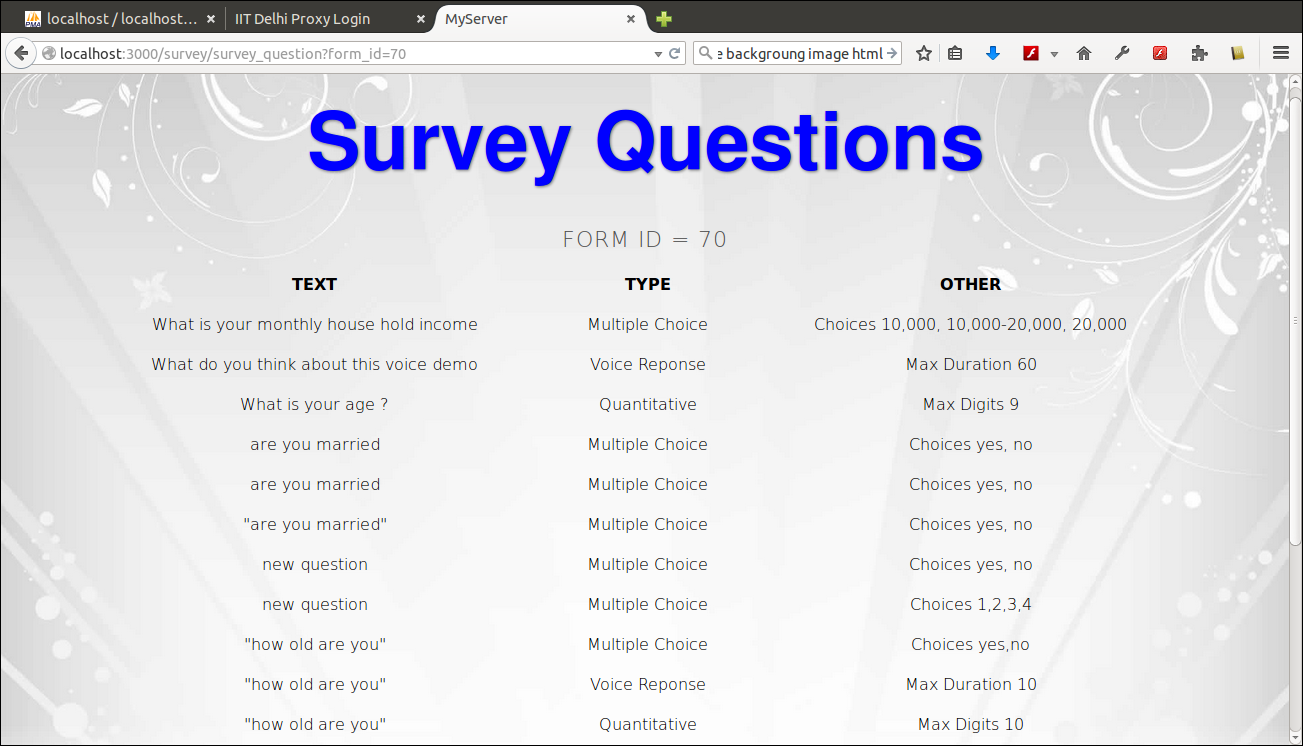
\includegraphics[scale=0.3]{w12}
\caption{View Active Survey Questions}
\label{fig:w12}
\end{center}
\end{figure}
 
\end{enumerate}
